\section{Guía de Uso}

	\subsection{Introducción}
		
		Esta sección pretende mostrar una vista general de la aplicación y sus opciones. A lo largo de ellan se explicarán todos los módulos del programa con los que el usuario tiene contacto y detallará la función de determinados mecanismos.\\
		
		\begin{figure}[htbp]
		\centering
		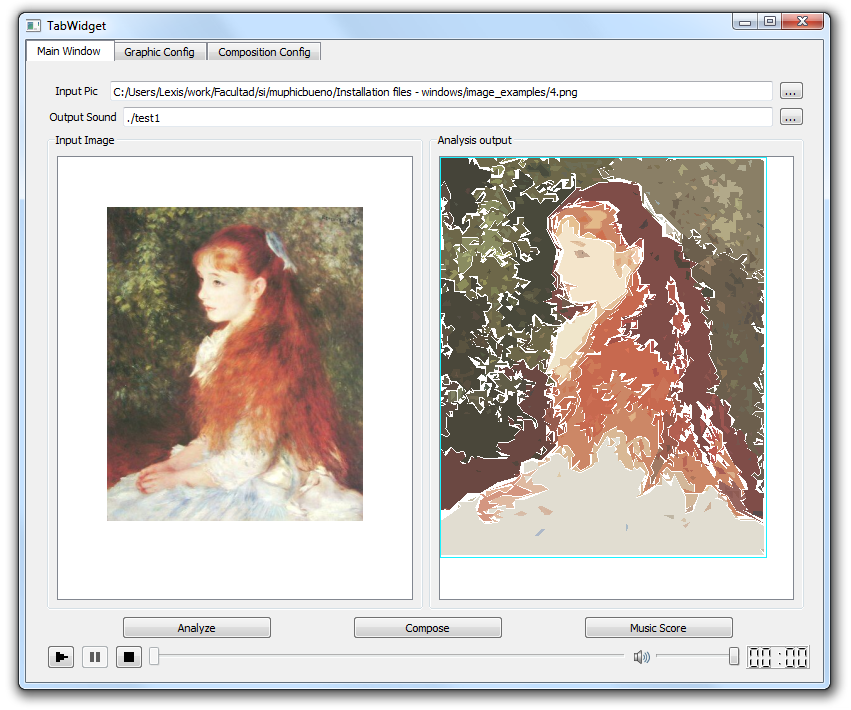
\includegraphics[scale=0.57]{graphics/interfazoverview.png}
		\caption{Vista general de la aplicación}
		\label{fig:interfazoverview}
		\end{figure}
		
		Como vemos en la Figura~\ref{fig:interfazoverview}, la aplicación dispone de 3 pestañas: Main Window, Graphic Config y Composition Config. La primera dispone de toda la funcionalidad necesaria para lanzar la aplicación, mientras que las otras 2 aportan opciones para configurar el comportamiento del análisis y la composición.\\
		
		De forma general, todo usuario, experto o inexperto, se puede valer de la primera pestaña para usar la composición. Sin embargo, un usuario avanzado con conocimientos musicales y de qué tipos de análisis gráficos se realizan puede navegar por las pestañas restantes para configurar el completo proceso mediante los parámetros ofrecidos.
		
		Se procede por tanto a explicar cada pestaña una por una.

	\subsection{Ventana principal}
		
		Se encarga de la interacción directa con el usuario; muestra los resultados obtenidos y permite lanzar los distintos componentes de la aplicación. 
		\\Esta compuesta por los siguientes elementos tal y como se puede ver en la Figura~\ref{fig:interfaz}:\\
		
		
		\begin{figure}[htbp]
		\centering
		\hspace*{-0.9in}
		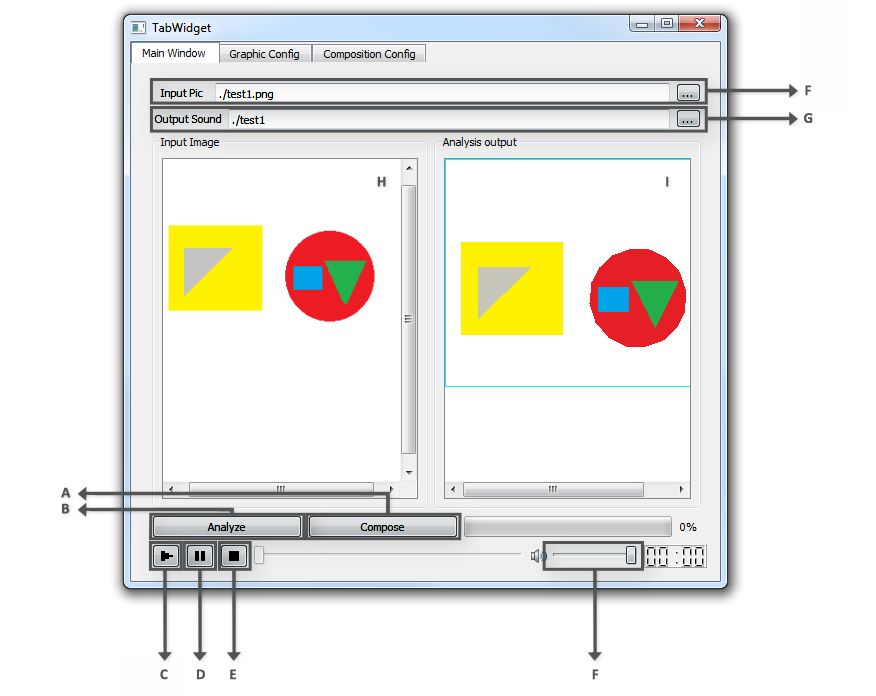
\includegraphics[scale=0.57]{graphics/interfaz.png}
		\caption{Vista general de la pestaña principal de la aplicación}
		\label{fig:interfaz}
		\end{figure}
		
		\noindent\textit{Carga de imagen de entrada [7]:}  Mediante esta opción el usuario puede elegir la dirección desde donde se cargará la imagen de entrada que se usará en el análisis. Para elegir la dirección podrá insertar el texto a mano o utilizar el botón para usar el explorador del sistema operativo correspondiente.\\
		
		\noindent\textit{Selección del archivo de audio de salida [8]:}  Mediante esta opción el usuario puede la dirección dodne se guardará el archivo de salida. Para elegir la dirección podrá insertar el texto a mano o utilizar el botón para usar el explorador del sistema operativo correspondiente.\\
		
		\noindent\textit{Input Image [A]:} En este panel se muestra la imagen elegida para el análisis.\\
		
		\noindent\textit{Analysis output [B]:} En este panel se muestra el resultado del último análisis realizado pulsando el botón "Analyze".\\
		
		\noindent\textit{Botón Analyze [2]:} Tal y como su nombre indica, Analyze, realiza el analisis de la imagen pasada como parámetro de entrada lanzando a ejecución el programa Phic, uno de los módulos de la aplicación. Tras analizarse, el resultado podrá observarse en el \textit{[B]}. Una vez pulsado el botón, y mientras dure el análisis, el botón pasará a mostrar el mensaje "STOP", pudiendo pulsarlo de nuevo para detener el análisis manualmente.\\
		
		\noindent\textit{Botón Compose [1]:} Realiza la composición musical a partir de los datos analizados, para ello lanza a ejecución el programa Mu, otro de los módulos de la aplicación. Una vez compuesta la pieza musical, se podrá escuchar mediante los controles de control de sonido. Una vez pulsado el botón, y mientras dure el análisis, el botón pasará a mostrar el mensaje "STOP", pudiendo pulsarlo de nuevo para detener la composición manualmente.\\
		
		\noindent\textit{Botón de Inicio de Reproducción [3]:} Permite al usuario iniciar la reproducción de la pieza musical compuesta por el módulo Mu.\\
		
		\noindent\textit{Botón de Pausa de Reproducción [4]:} Pausa la pieza musical en reproducción.\\
		
		\noindent\textit{Botón de Detención de Reproducción [5]:} Detiene la reproducción completamente.\\
		
		\noindent\textit{Barra de sonido [6]:} Modifica el volumen de la reproducción en curso.

		
	\subsection{Configuración gráfica}
		
		En esta pestaña se encuentran todas las opciones relacionadas con el análisis de la imagen. En ella se podrán configurar opciones que hagan que el proceso de análisis varíe en velocidad, precisión o estilo.\\
		
		De entre los parámetros de configuración, existen los llamados ``generales'', que siempre aparecen visibles al usuario, y los ``específicos'', que complementan a los generales y sólo aparecen cuando el contexto lo especifica. En la Figura~\ref{fig:interfazgraphic} podemos ver detalladamente los parámetros generales.\\
		
		\begin{figure}[htbp]
		\centering
		\hspace*{-0.9in}
		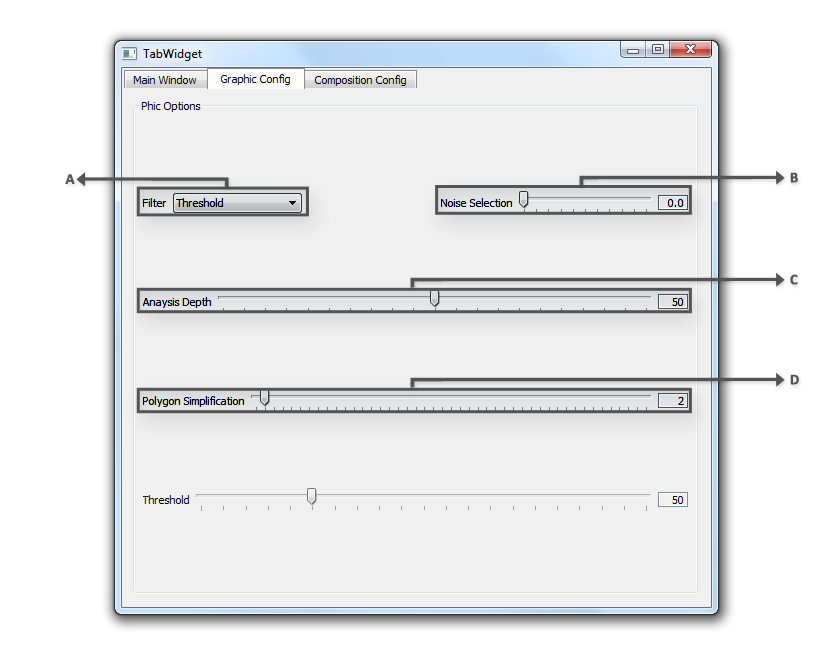
\includegraphics[scale=0.57]{graphics/interfazgraphic.png}
		\caption{Vista general de la pestaña de configuración gráfica}
		\label{fig:interfazgraphic}
		\end{figure}
		
		\noindent\textit{Tipo de filtrado de imagen [1]:} Distintos filtros en la imagen producirán diferentes formas de entender las formas que hay en ellas. De forma un poco más precisa, pero sin llegar a entrar en detalles técnicos, los filtros se encargan de transformar la imagen original a un mapa de bits en blanco y negro, que posteriormente se analizará para detectar polígonos en él. Un buen filtro diferenciará las deseadas superficies de color como manchas blancas independientes.\\
		
		\noindent\textit{Selección de ruido [2]:} Mediante esta barra el usuario puede elegir el tamaño mínimo de las formas por debajo del cual no se considerarán relevantes en el análisis. El valor representa un porcentaje respecto al area total de la imagen, de forma que un valor $n$ de Selección de Ruido determina que todas las formas con area menor a un $n$\% del area total de la imagen se considerarán ruido y no serán estudiadas.\\
		
		\noindent\textit{Profundidad del análisis [3]:} Permite variar el nivel de detalle con el que se realizará el análisis. Un valor de profundidad grande hará que el análisis se realice con gran parte los recursos que permite el programa (a costa de mayor lentitud en el análisis), mientras que un valores pequeños aumentarán la velocidad del proceso a costa de perder precisión a la hora de detectar formas de color.\\
		
		\noindent\textit{Simplificación de polígonos [4]:} Una vez detectadas las formas de color, es necesario aproximarlas a una lista de vértices para reducir el peso de la información sin modificar la carga de la misma. El nivel de fidelidad en la transformación de formas a polígonos se establece con este parámetro: un valor alto determina una gran fidelidad a costa de mayor tiempo de análisis, y viceversa.\\
		
		\noindent\textit{Botón Analyze [2]:} Tal y como su nombre indica, Analyze, realiza el analisis de la imagen pasada como parámetro de entrada lanzando a ejecución el programa Phic, uno de los módulos de la aplicación. Tras analizarse, el resultado podrá observarse en el \textit{[B]}.\\


		Los parámetros ``especícos'' dependen única y exclusivamente del tipo de filtro seleccionado [1], ya que cada tipo de filtro introduce nuevas opciones que configurar. \\
		
		
		Todo filtro en la aplicación que nos ocupa, como ya se comentó anteriormente, realizan la misma función: detectar formas y expresarlas como superficies blancas. A continuación se explica de forma general el funcionamiento de cada filtro y sus parámetros ``específicos''.\\
		
	\noindent\textbf{Threshold}\\
		
		\begin{figure}[htbp]
		\centering
		\hspace*{-0.9in}
		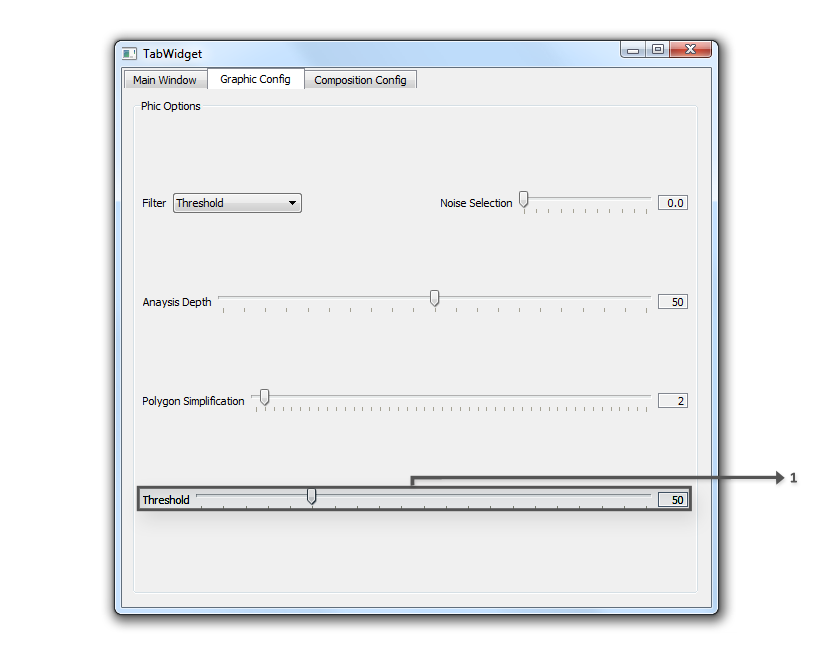
\includegraphics[scale=0.57]{graphics/interfazthreshold.png}
		\caption{Vista del filtro Threshold}
		\label{fig:interfazthreshold}
		\end{figure}
		
		Este filtro, contenido en varias librerías de procesado de imágenes (ver \cite{opencvDoc}), transforma la imagen a escala de grises para luego marcar como blancos todos los píxeles con un valor de gris superiores a un umbral dado, y como negros el resto.\\
		
		Los parámetros específicos que usa, vistos en la Figura~\ref{fig:interfazthreshold}, son:\\		
		
		\noindent\textit{Valor del umbral [1]:} Establece el valor del umbral antes explicado.\\
		
	\noindent\textbf{Adaptative Threshold}\\

		Mientras que el filtro anterior utiliza un mismo umbral para toda la imagen, Adaptative Threshold (ver \cite{opencvDoc}) analiza cada parte de la imagen en escala de grises y decide qué umbral es mejor para cada sección.\\ 
		
		Este filtro no usa parámetros específicos, ya que recalcula el valor del umbral cada vez que le resulta necesario.\\
		
	\noindent\textbf{Canny}\\

		Utiliza el algoritmo de detección de regiones del mismo nombre, desarrollado en 1986 por John F. Canny (ver \cite{opencvDoc}). Una vez encontrados los bordes, establece las figuras que estos delimitan.\\
		
		Este filtro no usa parámetros específicos.\\
		
	\noindent\textbf{Hue Division}\\

		\begin{figure}[htbp]
		\centering
		\hspace*{-0.9in}
		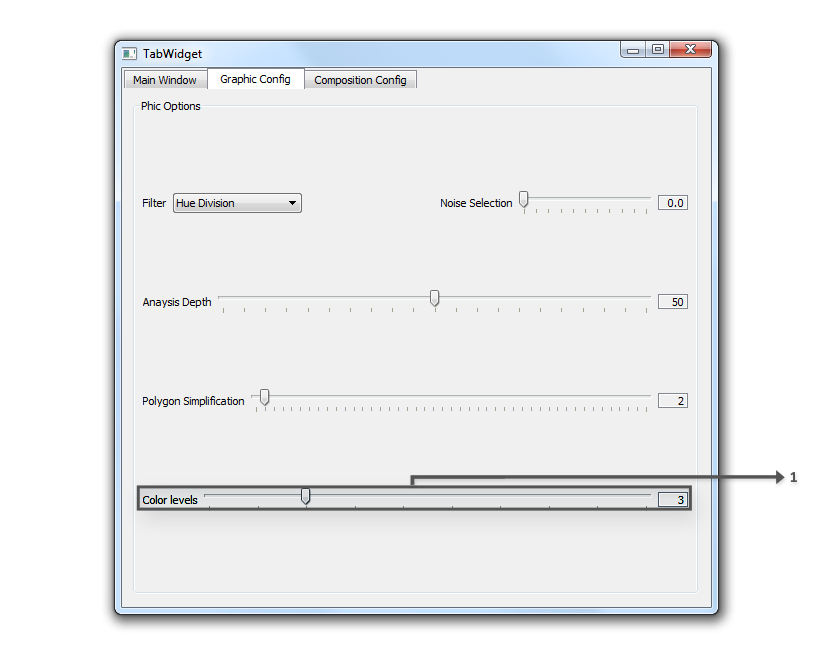
\includegraphics[scale=0.57]{graphics/interfazhue.png}
		\caption{Vista general del filtro Hue Division}
		\label{fig:interfazhue}
		\end{figure}

		Se trata de un filtro propio que busca asocia manchas de color con conjuntos de píxeles vecinos con valores RGB dentro de un mismo rango de rojo (R), azul (B) y verde (G). Los parámetros específicos son:\\
		
		\noindent\textit{Niveles de color[1]:} Este parámetro determina el número de intervalos posibles de color que puede haber en cada canal de color, y por tanto determinará la amplitud de cada rango. Un valor igual a 3 indica que un pixel cualquiera puede entrar dentro de 3 intervalos posibles en el canal rojo, otros 3 en el azul y otros 3 en el verde. De esta forma cada píxel entra dentro de una de las $3*3*3=27$ categorías de color, simplificando el análisis. Un valor muy grande de este parámetro hará que haya más categorías de color y que por tanto colores que antes se consideraban parte de una misma forma ahora se consideren como parte de formas independientes con colores más específicos. Un valor muy pequeño hará que se interpreten formas más amplias (incluyendo píxeles más diversos).\\
		
	\noindent\textbf{Color Threshold}\\

		\begin{figure}[htbp]
		\centering
		\hspace*{-0.9in}
		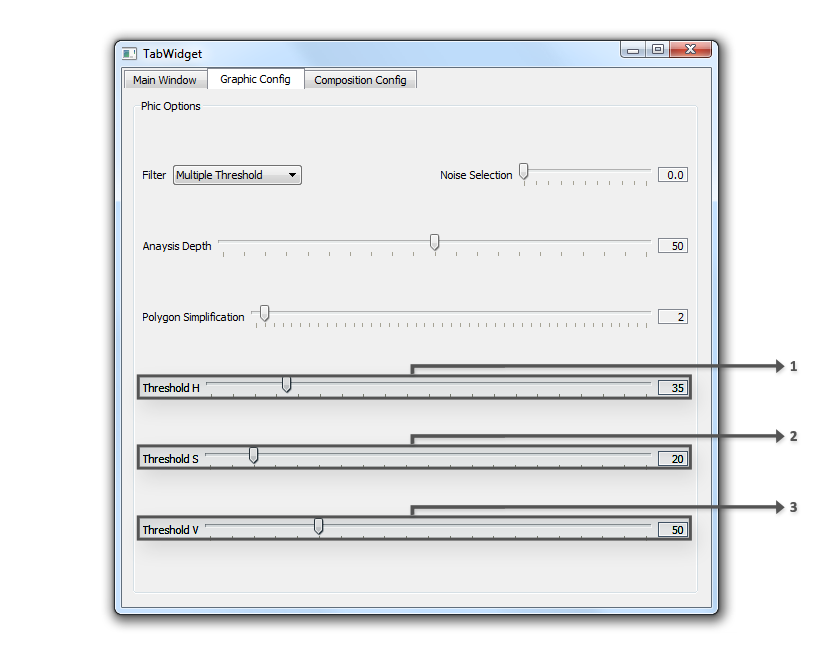
\includegraphics[scale=0.57]{graphics/interfaz3threshold.png}
		\caption{Vista general del filtro Color Threshold}
		\label{fig:interfaz3threshold}
		\end{figure}

		Se trata de un filtro propio que adapta el filtro Threshold para una imagen de 3 canales. En vez de considerar como figuras aquellas agrupaciones de píxeles cuyos valores en escala de grises sean inferiores a un umbral, considera aquellas que en su canal de Matiz (Hue), Saturación (Saturation) y Valor (Value) sean menor que un umbral, originando cada canal formas independientes.\\
		
		Los parámetros específicos de este filtro determinarán el valor de los umbrales de cada canal determinado en formato de imagen HSV.\\		
		
		\noindent\textit{Valor del umbral de Matiz[1]}\\
		\noindent\textit{Valor del umbral de Saturación[2]}\\
		\noindent\textit{Valor del umbral de Valor[3]}




		
		\subsubsection{Configuración de composición}
		
		Esta pestaña contiene todos los parámetros configurables relativos a la composición algoritmica. Estos, como muestra la Figura~\ref{fig:interfazcomp} son:\\
		
		\begin{figure}[htbp]
		\centering
		\hspace*{-0.9in}
		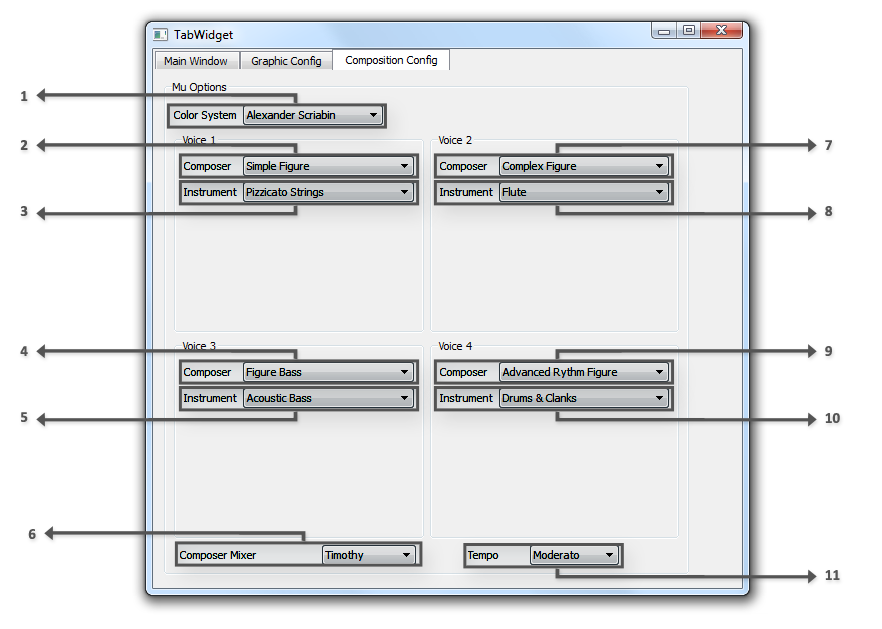
\includegraphics[scale=0.57]{graphics/interfazcomp.png}
		\caption{Vista general de la pestaña de configuración gráfica}
		\label{fig:interfazcomp}
		\end{figure}
		
		\noindent\textit{Sistema de color[1]:} Permite alternar entre las diferentes relaciones tono-color explicadas en el Capítulo~\ref{sec:algcomp}.\\
		
		\noindent\textit{Algoritmo de composición para la primera voz[2]:} Con esta opción, el usuario puede elegir, de entre los distintos algoritmos de composición, el que se usará para que generar la melodía principal.\\
		
		\noindent\textit{Algoritmo de composición para la segunda voz[7]:} Con esta opción, el usuario puede elegir, de entre los distintos algoritmos de composición, el que se usará para que generar la segunda melodía principal.\\

		\noindent\textit{Algoritmo de composición para la tercera voz[4]:} Con esta opción, el usuario puede elegir, de entre los distintos algoritmos de composición del bajo, el que se usará para que generar el bajo armónico.\\
		
		\noindent\textit{Algoritmo de composición para la cuarta voz[9]:} Con esta opción, el usuario puede elegir, de entre los distintos algoritmos de composición de ritmos, el que se usará para que generar el ritmo de la pieza musical final.\\
		
		\noindent\textit{Selección de instrumentos [3], [5], [8] y [10]:} Permiten seleccionar los instrumentos con los que sonaran las distintas voces.\\

		\noindent\textit{Algoritmo de composición general[6]:} Determina qué algoritmo se usará para recorrer la imagen y aplicar los algoritmos de las distintas voces. Se explica con detalle en el Capítulo~\ref{sec:algcomp}.\\

		\noindent\textit{Tempo[11]:} Como su nombre indica, su valor determina el tempo con el que sonará la pieza musical compuesta.\\
		
	\subsection{Requisitos de instalación}
	
		Muphic es una aplicación multiplaforma con soporte para Linux y Windows de 32 y 64 bits, siendo en ambos una aplicación portable. Para finalizar este capítulo, se detallará a continuación las peculiaridades de ejecución en cada plataforma.
		
		\subsubsection{Windows}
		
		Para ejecutar la aplicación basta con descomprimir el archivo descargado y ejecutar la aplicación.
		
		\subsubsection{Linux}
		
		Para utilizar la aplicación en cualquier distribución de Linux, habrá que descomprimir el archivo y generar los ejecutables con la herramienta make. Ciertos elementos del sistema (la interfaz gráfica y los controles de reproducción de sonido) requieren que el usuario tenga instaladas ciertas librerías que no se incluyen en la descarga de la aplicación. Estos paquetes son:
		
		\begin{itemize}
			\item Librerías de qt versión 4.7.4, disponibles en su página web (ver \cite{qtlibs}).		
			\item \emph{libphonon-dev (multimedia framework from KDE-development files)} 
			\item \emph{libphonon4 (multimedia framework from KDE-core library)}
			\item \emph{phonon (multimedia framework from KDE-metapackage)}
			\item \emph{phonon-backend-gstreamer (Phonon GStreamer 0.10.x backend)}
			\item \emph{libqt4script4-phonon (Qt Script bindings for the Qt 4 Phonon library)}
			
		\end{itemize}
	
		Si el paquete \emph{phonon-backend-gstreamer}, por cualquier razón, fuera el origen de algún fallo; el usario puede elegir probar con otros tipos de backend, como por ejemplo \emph{phonon-backend-vlc}.
		
		
		\todo{probar en Mac, que es UNIX y no hay razón por la que no deba ir}